
%% bare_conf.tex
%% V1.3
%% 2007/01/11
%% by Michael Shell
%% See:
%% http://www.michaelshell.org/
%% for current contact information.
%%
%% This is a skeleton file demonstrating the use of IEEEtran.cls
%% (requires IEEEtran.cls version 1.7 or later) with an IEEE conference paper.
%%
%% Support sites:
%% http://www.michaelshell.org/tex/ieeetran/
%% http://www.ctan.org/tex-archive/macros/latex/contrib/IEEEtran/
%% and
%% http://www.ieee.org/

%%*************************************************************************
%% Legal Notice:
%% This code is offered as-is without any warranty either expressed or
%% implied; without even the implied warranty of MERCHANTABILITY or
%% FITNESS FOR A PARTICULAR PURPOSE! 
%% User assumes all risk.
%% In no event shall IEEE or any contributor to this code be liable for
%% any damages or losses, including, but not limited to, incidental,
%% consequential, or any other damages, resulting from the use or misuse
%% of any information contained here.
%%
%% All comments are the opinions of their respective authors and are not
%% necessarily endorsed by the IEEE.
%%
%% This work is distributed under the LaTeX Project Public License (LPPL)
%% ( http://www.latex-project.org/ ) version 1.3, and may be freely used,
%% distributed and modified. A copy of the LPPL, version 1.3, is included
%% in the base LaTeX documentation of all distributions of LaTeX released
%% 2003/12/01 or later.
%% Retain all contribution notices and credits.
%% ** Modified files should be clearly indicated as such, including  **
%% ** renaming them and changing author support contact information. **
%%
%% File list of work: IEEEtran.cls, IEEEtran_HOWTO.pdf, bare_adv.tex,
%%                    bare_conf.tex, bare_jrnl.tex, bare_jrnl_compsoc.tex
%%*************************************************************************

% *** Authors should verify (and, if needed, correct) their LaTeX system  ***
% *** with the testflow diagnostic prior to trusting their LaTeX platform ***
% *** with production work. IEEE's font choices can trigger bugs that do  ***
% *** not appear when using other class files.                            ***
% The testflow support page is at:
% http://www.michaelshell.org/tex/testflow/



% Note that the a4paper option is mainly intended so that authors in
% countries using A4 can easily print to A4 and see how their papers will
% look in print - the typesetting of the document will not typically be
% affected with changes in paper size (but the bottom and side margins will).
% Use the testflow package mentioned above to verify correct handling of
% both paper sizes by the user's LaTeX system.
%
% Also note that the "draftcls" or "draftclsnofoot", not "draft", option
% should be used if it is desired that the figures are to be displayed in
% draft mode.
%
\documentclass[conference]{IEEEtran}
\usepackage{blindtext, graphicx}
\usepackage{float}
% Add the compsoc option for Computer Society conferences.
%
% If IEEEtran.cls has not been installed into the LaTeX system files,
% manually specify the path to it like:
% \documentclass[conference]{../sty/IEEEtran}





% Some very useful LaTeX packages include:
% (uncomment the ones you want to load)


% *** MISC UTILITY PACKAGES ***
%
%\usepackage{ifpdf}
% Heiko Oberdiek's ifpdf.sty is very useful if you need conditional
% compilation based on whether the output is pdf or dvi.
% usage:
% \ifpdf
%   % pdf code
% \else
%   % dvi code
% \fi
% The latest version of ifpdf.sty can be obtained from:
% http://www.ctan.org/tex-archive/macros/latex/contrib/oberdiek/
% Also, note that IEEEtran.cls V1.7 and later provides a builtin
% \ifCLASSINFOpdf conditional that works the same way.
% When switching from latex to pdflatex and vice-versa, the compiler may
% have to be run twice to clear warning/error messages.






% *** CITATION PACKAGES ***
%
%\usepackage{cite}
% cite.sty was written by Donald Arseneau
% V1.6 and later of IEEEtran pre-defines the format of the cite.sty package
% \cite{} output to follow that of IEEE. Loading the cite package will
% result in citation numbers being automatically sorted and properly
% "compressed/ranged". e.g., [1], [9], [2], [7], [5], [6] without using
% cite.sty will become [1], [2], [5]--[7], [9] using cite.sty. cite.sty's
% \cite will automatically add leading space, if needed. Use cite.sty's
% noadjust option (cite.sty V3.8 and later) if you want to turn this off.
% cite.sty is already installed on most LaTeX systems. Be sure and use
% version 4.0 (2003-05-27) and later if using hyperref.sty. cite.sty does
% not currently provide for hyperlinked citations.
% The latest version can be obtained at:
% http://www.ctan.org/tex-archive/macros/latex/contrib/cite/
% The documentation is contained in the cite.sty file itself.






% *** GRAPHICS RELATED PACKAGES ***
%
\ifCLASSINFOpdf
  % \usepackage[pdftex]{graphicx}
  % declare the path(s) where your graphic files are
  % \graphicspath{{../pdf/}{../jpeg/}}
  % and their extensions so you won't have to specify these with
  % every instance of \includegraphics
  % \DeclareGraphicsExtensions{.pdf,.jpeg,.png}
\else
  % or other class option (dvipsone, dvipdf, if not using dvips). graphicx
  % will default to the driver specified in the system graphics.cfg if no
  % driver is specified.
  % \usepackage[dvips]{graphicx}
  % declare the path(s) where your graphic files are
  % \graphicspath{{../eps/}}
  % and their extensions so you won't have to specify these with
  % every instance of \includegraphics
  % \DeclareGraphicsExtensions{.eps}
\fi
% graphicx was written by David Carlisle and Sebastian Rahtz. It is
% required if you want graphics, photos, etc. graphicx.sty is already
% installed on most LaTeX systems. The latest version and documentation can
% be obtained at: 
% http://www.ctan.org/tex-archive/macros/latex/required/graphics/
% Another good source of documentation is "Using Imported Graphics in
% LaTeX2e" by Keith Reckdahl which can be found as epslatex.ps or
% epslatex.pdf at: http://www.ctan.org/tex-archive/info/
%
% latex, and pdflatex in dvi mode, support graphics in encapsulated
% postscript (.eps) format. pdflatex in pdf mode supports graphics
% in .pdf, .jpeg, .png and .mps (metapost) formats. Users should ensure
% that all non-photo figures use a vector format (.eps, .pdf, .mps) and
% not a bitmapped formats (.jpeg, .png). IEEE frowns on bitmapped formats
% which can result in "jaggedy"/blurry rendering of lines and letters as
% well as large increases in file sizes.
%
% You can find documentation about the pdfTeX application at:
% http://www.tug.org/applications/pdftex





% *** MATH PACKAGES ***
%
%\usepackage[cmex10]{amsmath}
% A popular package from the American Mathematical Society that provides
% many useful and powerful commands for dealing with mathematics. If using
% it, be sure to load this package with the cmex10 option to ensure that
% only type 1 fonts will utilized at all point sizes. Without this option,
% it is possible that some math symbols, particularly those within
% footnotes, will be rendered in bitmap form which will result in a
% document that can not be IEEE Xplore compliant!
%
% Also, note that the amsmath package sets \interdisplaylinepenalty to 10000
% thus preventing page breaks from occurring within multiline equations. Use:
%\interdisplaylinepenalty=2500
% after loading amsmath to restore such page breaks as IEEEtran.cls normally
% does. amsmath.sty is already installed on most LaTeX systems. The latest
% version and documentation can be obtained at:
% http://www.ctan.org/tex-archive/macros/latex/required/amslatex/math/





% *** SPECIALIZED LIST PACKAGES ***
%
%\usepackage{algorithmic}
% algorithmic.sty was written by Peter Williams and Rogerio Brito.
% This package provides an algorithmic environment fo describing algorithms.
% You can use the algorithmic environment in-text or within a figure
% environment to provide for a floating algorithm. Do NOT use the algorithm
% floating environment provided by algorithm.sty (by the same authors) or
% algorithm2e.sty (by Christophe Fiorio) as IEEE does not use dedicated
% algorithm float types and packages that provide these will not provide
% correct IEEE style captions. The latest version and documentation of
% algorithmic.sty can be obtained at:
% http://www.ctan.org/tex-archive/macros/latex/contrib/algorithms/
% There is also a support site at:
% http://algorithms.berlios.de/index.html
% Also of interest may be the (relatively newer and more customizable)
% algorithmicx.sty package by Szasz Janos:
% http://www.ctan.org/tex-archive/macros/latex/contrib/algorithmicx/




% *** ALIGNMENT PACKAGES ***
%
%\usepackage{array}
% Frank Mittelbach's and David Carlisle's array.sty patches and improves
% the standard LaTeX2e array and tabular environments to provide better
% appearance and additional user controls. As the default LaTeX2e table
% generation code is lacking to the point of almost being broken with
% respect to the quality of the end results, all users are strongly
% advised to use an enhanced (at the very least that provided by array.sty)
% set of table tools. array.sty is already installed on most systems. The
% latest version and documentation can be obtained at:
% http://www.ctan.org/tex-archive/macros/latex/required/tools/


%\usepackage{mdwmath}
%\usepackage{mdwtab}
% Also highly recommended is Mark Wooding's extremely powerful MDW tools,
% especially mdwmath.sty and mdwtab.sty which are used to format equations
% and tables, respectively. The MDWtools set is already installed on most
% LaTeX systems. The lastest version and documentation is available at:
% http://www.ctan.org/tex-archive/macros/latex/contrib/mdwtools/


% IEEEtran contains the IEEEeqnarray family of commands that can be used to
% generate multiline equations as well as matrices, tables, etc., of high
% quality.


%\usepackage{eqparbox}
% Also of notable interest is Scott Pakin's eqparbox package for creating
% (automatically sized) equal width boxes - aka "natural width parboxes".
% Available at:
% http://www.ctan.org/tex-archive/macros/latex/contrib/eqparbox/





% *** SUBFIGURE PACKAGES ***
%\usepackage[tight,footnotesize]{subfigure}
% subfigure.sty was written by Steven Douglas Cochran. This package makes it
% easy to put subfigures in your figures. e.g., "Figure 1a and 1b". For IEEE
% work, it is a good idea to load it with the tight package option to reduce
% the amount of white space around the subfigures. subfigure.sty is already
% installed on most LaTeX systems. The latest version and documentation can
% be obtained at:
% http://www.ctan.org/tex-archive/obsolete/macros/latex/contrib/subfigure/
% subfigure.sty has been superceeded by subfig.sty.



%\usepackage[caption=false]{caption}
%\usepackage[font=footnotesize]{subfig}
% subfig.sty, also written by Steven Douglas Cochran, is the modern
% replacement for subfigure.sty. However, subfig.sty requires and
% automatically loads Axel Sommerfeldt's caption.sty which will override
% IEEEtran.cls handling of captions and this will result in nonIEEE style
% figure/table captions. To prevent this problem, be sure and preload
% caption.sty with its "caption=false" package option. This is will preserve
% IEEEtran.cls handing of captions. Version 1.3 (2005/06/28) and later 
% (recommended due to many improvements over 1.2) of subfig.sty supports
% the caption=false option directly:
%\usepackage[caption=false,font=footnotesize]{subfig}
%
% The latest version and documentation can be obtained at:
% http://www.ctan.org/tex-archive/macros/latex/contrib/subfig/
% The latest version and documentation of caption.sty can be obtained at:
% http://www.ctan.org/tex-archive/macros/latex/contrib/caption/




% *** FLOAT PACKAGES ***
%
%\usepackage{fixltx2e}
% fixltx2e, the successor to the earlier fix2col.sty, was written by
% Frank Mittelbach and David Carlisle. This package corrects a few problems
% in the LaTeX2e kernel, the most notable of which is that in current
% LaTeX2e releases, the ordering of single and double column floats is not
% guaranteed to be preserved. Thus, an unpatched LaTeX2e can allow a
% single column figure to be placed prior to an earlier double column
% figure. The latest version and documentation can be found at:
% http://www.ctan.org/tex-archive/macros/latex/base/



%\usepackage{stfloats}
% stfloats.sty was written by Sigitas Tolusis. This package gives LaTeX2e
% the ability to do double column floats at the bottom of the page as well
% as the top. (e.g., "\begin{figure*}[!b]" is not normally possible in
% LaTeX2e). It also provides a command:
%\fnbelowfloat
% to enable the placement of footnotes below bottom floats (the standard
% LaTeX2e kernel puts them above bottom floats). This is an invasive package
% which rewrites many portions of the LaTeX2e float routines. It may not work
% with other packages that modify the LaTeX2e float routines. The latest
% version and documentation can be obtained at:
% http://www.ctan.org/tex-archive/macros/latex/contrib/sttools/
% Documentation is contained in the stfloats.sty comments as well as in the
% presfull.pdf file. Do not use the stfloats baselinefloat ability as IEEE
% does not allow \baselineskip to stretch. Authors submitting work to the
% IEEE should note that IEEE rarely uses double column equations and
% that authors should try to avoid such use. Do not be tempted to use the
% cuted.sty or midfloat.sty packages (also by Sigitas Tolusis) as IEEE does
% not format its papers in such ways.





% *** PDF, URL AND HYPERLINK PACKAGES ***
%
%\usepackage{url}
% url.sty was written by Donald Arseneau. It provides better support for
% handling and breaking URLs. url.sty is already installed on most LaTeX
% systems. The latest version can be obtained at:
% http://www.ctan.org/tex-archive/macros/latex/contrib/misc/
% Read the url.sty source comments for usage information. Basically,
% \url{my_url_here}.





% *** Do not adjust lengths that control margins, column widths, etc. ***
% *** Do not use packages that alter fonts (such as pslatex).         ***
% There should be no need to do such things with IEEEtran.cls V1.6 and later.
% (Unless specifically asked to do so by the journal or conference you plan
% to submit to, of course. )


% correct bad hyphenation here
\hyphenation{op-tical net-works semi-conduc-tor}


\begin{document}
%
% paper title
% can use linebreaks \\ within to get better formatting as desired
\title{Multilingual Sentiment based Review Summarizer}


% author names and affiliations
% use a multiple column layout for up to three different
% affiliations
\author{\IEEEauthorblockN{Siddharth Dasani}
\IEEEauthorblockA{8209990799\\
sdasani@usc.edu}
\and
\IEEEauthorblockN{Piyush Gupta}
\IEEEauthorblockA{2344499379\\
piyush@usc.edu}
\and
\IEEEauthorblockN{Susanth Dahal}
\IEEEauthorblockA{ 7553849598\\
dahal@usc.edu}
\and
\IEEEauthorblockN{Dishant Shahani}
\IEEEauthorblockA{4798718230\\
dshahani@usc.edu}}

% conference papers do not typically use \thanks and this command
% is locked out in conference mode. If really needed, such as for
% the acknowledgment of grants, issue a \IEEEoverridecommandlockouts
% after \documentclass

% for over three affiliations, or if they all won't fit within the width
% of the page, use this alternative format:
% 
%\author{\IEEEauthorblockN{Michael Shell\IEEEauthorrefmark{1},
%Homer Simpson\IEEEauthorrefmark{2},
%James Kirk\IEEEauthorrefmark{3}, 
%Montgomery Scott\IEEEauthorrefmark{3} and
%Eldon Tyrell\IEEEauthorrefmark{4}}
%\IEEEauthorblockA{\IEEEauthorrefmark{1}School of Electrical and Computer Engineering\\
%Georgia Institute of Technology,
%Atlanta, Georgia 30332--0250\\ Email: see http://www.michaelshell.org/contact.html}
%\IEEEauthorblockA{\IEEEauthorrefmark{2}Twentieth Century Fox, Springfield, USA\\
%Email: homer@thesimpsons.com}
%\IEEEauthorblockA{\IEEEauthorrefmark{3}Starfleet Academy, San Francisco, California 96678-2391\\
%Telephone: (800) 555--1212, Fax: (888) 555--1212}
%\IEEEauthorblockA{\IEEEauthorrefmark{4}Tyrell Inc., 123 Replicant Street, Los Angeles, California 90210--4321}}




% use for special paper notices
%\IEEEspecialpapernotice{(Invited Paper)}




% make the title area
\maketitle


% For peer review papers, you can put extra information on the cover
% page as needed:
% \ifCLASSOPTIONpeerreview
% \begin{center} \bfseries EDICS Category: 3-BBND \end{center}
% \fi
%
% For peerreview papers, this IEEEtran command inserts a page break and
% creates the second title. It will be ignored for other modes.
\IEEEpeerreviewmaketitle

\section{\textbf{Introduction}}
\subsection{\textbf{Description of the problem \& proposed solution}}
\indent We, as humans, have a natural inclination towards opinions. While purchasing a new product or looking for a new restaurant, we always seek and consider others opinion. With the rapid growth of e-commerce and review websites, there is a huge size of review corpus the users are exposed to. Also the websites currently provide only an absolute rating for a product or service without describing its individual features. For a user to identify the positive and negative features of a product, one would have to do the arduous task of going over all the reviews. Our project aims to solve this problem by generating a concise sentiment based summary which would provide the users with a holistic idea of a product$'$s features.\\\\
\indent In this project, given a large review corpus in French or German, we aim to identify the significant features and respective descriptors from a product$'$s reviews. Furthermore, we use a sentiment classifier to classify the pairs as positives or negatives of a product and finally use semantic analysis to display the pairs in the order of relevancy. This provides a user with a comprehensive summary regarding a product$’$s features which could prove helpful in making a buying decision.
\subsection{\textbf{Why is it interesting \& our contribution}}
\indent This project is interesting because nowadays as the amount of data available is enormous, the task of managing and interpreting the information is gaining significance. This process  of sentiment based summarization of a data corpus can be used not only for product reviews but also for summarizing books, news articles, magazines etc. and in domains like feature based information retrival. Moreover we decided to design it to work for multilingual corpora(currently French \& German). This would enable us to provide a clear summarization of a given subject or product irrespective of the data source language.\\\\
\indent The task was technically challenging because while extracting the relevant feature-descriptor pairs, identifying only the nouns-adjective phrases using POS tagging was not sufficient. We had to perform dependency parsing to identify which noun a given adjective describes. Finally as a contribution to current work, most existing summarizers take only the frequency of features into account, but in our implementation we consider semantic similarity as well to identify relevancy. We also perform sentiment based classification which helps to classify the feature-descriptors pairs as positive or negative.

\section{\textbf{Data Source \& Annotations}}
\indent We used Webis-CLS-10 corpora available through The Bauhaus-University$'$s website. The Cross-Lingual Sentiment(CLS) dataset was first used in Prettenhofer and Stein (2010). It comprises of Amazon reviews for Books, Dvd$'$s and Music in four languages (French, German, Japanese, English). It consisted of around 70000 reviews in each language.We currently implemented a summarizer for French \& German.

\indent The data was available as a raw XML file. Each review was represented by an $<$item$>$ element. Each $<$item$>$ element has following child elements: \begin{enumerate} \item category: The product category. \item rating: The number of stars (1-5). \item url: The url of the webpage from which the review was fetched.\item text: The review text. \item title: The name of the product.\item reviewer: The name of the author. \item location: The location of the author (may be empty). \item date: The date when the review was written.\end{enumerate}
\indent The above structure was same for both the languages, French \& German. As an input to our implementation we give a folder having reviews in both languages. We use a python language detection library to identify the language. Out of the above given tags, we used the content under the $<$Text$>$ and $<$Title$>$ tags for the purpose of this project. For a given specific $<$Title$>$ we used a dictionary to aggregate all the reviews written by all reviewers into one list. This made a specific product$’$s reviews easily available to work with. Although the available review dataset was pre-annotated with a sentiment label classifying the whole review as positive or negative, it was not useful in our sentiment analysis task because there can be a case when a review consists of many positive features of a product but the overall sentiment of the review is negative. eg: "It has a great camera but not worth the money".\\
\indent Our task was to identify feature-descriptor pairs and classify them as positives or negatives for a given product. For the purpose of evaluation, as the pre-annotated review sentiment was  not helpful, we filtered out a subset of 2000 reviews, 1000 in french \& 1000 in German.  We translated them to english using Google translate. We then manually identified the positive and negative feature-descriptor pairs from the translated reviews. We use this as a reference solution and compare our output with this reference using the F1 score measure.\\\\\\\\\\

\section{\textbf{Procedure}}
\subsection{\textbf{Data Preprocessing}}
\indent Initially as we were dealing with two languages (French \& German), we used the python package \textbf{langdetect} to identify the language of a given review text. This helped us segregate the reviews based on language. We then need to identify the significant features of a given product from reviews. Most of the features of a particular product generally occur in the reviews as Nouns and Noun Phrases. The opinion about these features are adjectives that describe these features. We use \textbf{pattern.fr} and \textbf{pattern.de} python libraries developed by CLiPS(Computational Linguistics And Psycholinguistics) to perform POS tagging for french and German reviews respectively. This helped us to identify the Nouns and Adjectives in the sentence. 
\subsection{\textbf{Dependency Parsing}}
\indent We noticed that in many reviews the product name was replaced by a pronoun. So in this part, we replaced the pronoun with the Noun it refers to. For this purpose we used the \textbf{parsetree} function available in pattern library. It generates the parse tree of a sentence and extract typed dependencies showing the grammatical relationships among the words. This helped to identify which noun a given pronoun is referring to. Furthermore, for a sentence having multiple feature-descriptor pairs, in order to identify which Noun a given Adjective modifies, we used the same dependency parsing using the the parsetree function of the pattern library.
\subsection{\textbf{Sentiment based classification \& Filtering}}
\indent Now that we have extracted the related feature-descriptor pairs, the next part is getting the sentiment of each pair of phrases.This would help us to classify the specific feature as positive or negative. For this task, we used the sentiment function of the pattern.fr and pattern.de library for french and german respectivelty. The function returns a value between [-1, 1] where values less than 0 represents negative sentiment and value more than 0 represent positive sentiment. In order to filter out less relevant pairs, we defined the threshold value of [-0.2, 0.2] and disregarded the pairs having sentiment value in this range. 
\subsection{\textbf{Sorting features using Semantic Similarity}}
\indent Finally having obtained the positive and negative features-descriptor pairs for a product, we need to sort them based on the relevancy of the subject. To do that we take into account their semantic similarity. For this task, we use a Java API called \textbf{DISCO} that is available as a precompiled jar and can be queried through the terminal. We have to give the string as a parameter along with the similarity measure to be used. We used the COSINE similarity measure as it provided most relevant results for the sample reviews. Having obtained the semantic similarity value for each pair, we use it as a measure to sort the positive and negative features in a descending order of their similarity value. These sorted pairs of phrases within positives and negatives are then presented to the user if form of a word cloud.
\begin{figure}[H]
\centering
\includegraphics[width=8.5cm, height=7.5cm]{flowchart.png}
\end{figure}

\section{\textbf{Evaluation}}
\indent As a final output we get feature-descriptor pairs classified into positives and negatives group and sorted according to relevance based on the semantic similarity value. In order to compare our results with the program output, we took a sample of 2000 reviews and manually created a summary in form of product features. For the sample dataset, we measure it$'$s performance by taking into account the following factors:
\begin{enumerate}
\item The number of features correctly identified by the model.
\item The correctness in terms of identifying the sentiment of a feature by the model.\end{enumerate}
\subsection{\textbf{Evaluation - Feature Identification}}
\indent We have Used F-Score to measure the performance of our model in terms of feature detection. Let the number of correct features identified by the model be $N_{cf}$  and the total number of features identified be $N_{tf}$ . Also, let $N_{f}$ be the correct number of features in the overall reviews of a product which we identified manually. Now we define the Precision of identified features, $P_{f}$ as the ratio of the number of correct features identified by the model and the total number of features identified by the model.
$$P_{f}=\frac{N_{cf}}{N_{tf}}$$We have defined the Recall of identified features, $R_{f}$ as the ratio of the number of correct features identified by the model and the actual number of correct features in all the reviews for the product.(annotated manually).$$R_{f}=\frac{N_{cf}}{N_{f}}$$
Hence the F-Score of  identified features, $F_{s}$ can hence be calculated as:
$$F_{s}=\frac{2P_{f}R_{f}}{P_{f}+R_{f}}$$
\subsection{\textbf{ Evaluation - Sentiment Analysis}}
\indent Let $N_{tp}$ be the number of correctly identified positive features, $N_{fp}$ be the number of negative features classified as positive, $N_{tn}$ be the number of correctly identified negative features and $N_{fn}$ be the number of positive features classified as negative.
As in the previous section, we define the precision ($P_{p}$), recall ($R_{p}$) and F-Score ($F_{p}$) to be,
$$P_{p}=\frac{N_{tp}}{N_{tp}+N_{fp}}$$
$$R_{p}=\frac{N_{tp}}{N_{tp}+N_{fn}}$$
$$F_{p}=\frac{2P_{p}R_{p}}{P_{p}+R_{p}}$$
Similarly, for negatively classified subjects, we define the precision ($P_{n}$), recall ($R_{n}$) and F-score ($F_{n}$) to be,
$$P_{n}=\frac{N_{tn}}{N_{tn}+N_{fn}}$$
$$R_{n}=\frac{N_{tn}}{N_{tn}+N_{fp}}$$
$$F_{n}=\frac{2P_{n}R_{n}}{P_{n}+R_{n}}$$
\section{\textbf{Results}}
\subsection{\textbf{Performance Measure}}
\indent In order to evaluate the performance, we have manually annotated data for both the languages (French \& German). We used 2000 manually annotated reviews, 1000 in each language, and used it as a baseline to find the F-score for our implementation. 
The precision, recall and F-Score values for the French data set of Books, Dvd$'$s and Music combined are given as:
\begin{center}
\begin{tabular}{ |c|c|c|c|  }
 \hline
 & Features & Positives & Negatives\\
 \hline
 Precision & 0.75 & 0.77 & 0.75\\
Recall & 0.73 & 0.76 & 0.72\\
F-Score & 0.74 & 0.76 & 0.73\\
 \hline
\end{tabular}
\end{center}
\indent The precision, recall and F-Score values for the German data set of Books, Dvd$'$s and Music combined are given as:
\begin{center}
\begin{tabular}{ |c|c|c|c|  }
 \hline
 & Features & Positives & Negatives\\
 \hline
 Precision & 0.71 & 0.73 & 0.70\\
Recall & 0.69 & 0.74 & 0.67\\
F-Score & 0.69 & 0.74 & 0.68\\
 \hline
\end{tabular}
\end{center}
Sample wordclouds showing positive and negative features of a specific DVD  are shown below. Their corresponding english translation is also shown for reference.

\begin{figure}[H]
\centering
\caption{Sample wordcloud for Positive Reviews (French)}
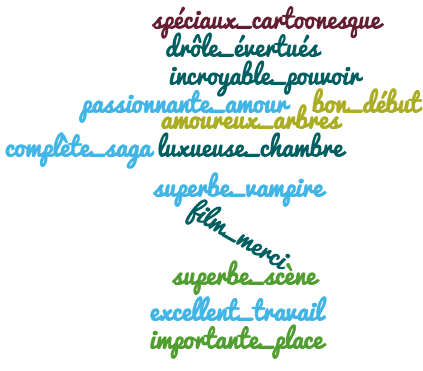
\includegraphics[width=7cm, height=5cm]{positive.png}
\end{figure}
\begin{figure}[H]
\centering
\caption{Sample wordcloud for Positive Reviews (English)}
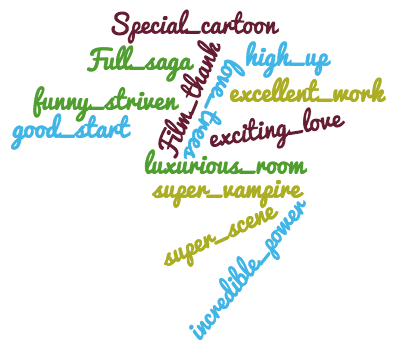
\includegraphics[width=7cm, height=5cm]{positive_en.png}
\end{figure}
\begin{figure}[H]
\centering
\caption{Sample wordcloud for Negative Reviews (French)}
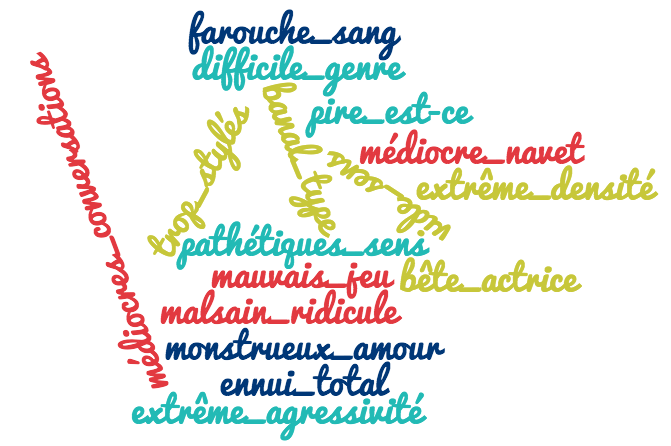
\includegraphics[width=7cm, height=5cm]{negative.png}
\end{figure}
\begin{figure}[H]
\centering
\caption{Sample wordcloud for Negative Reviews (English)}
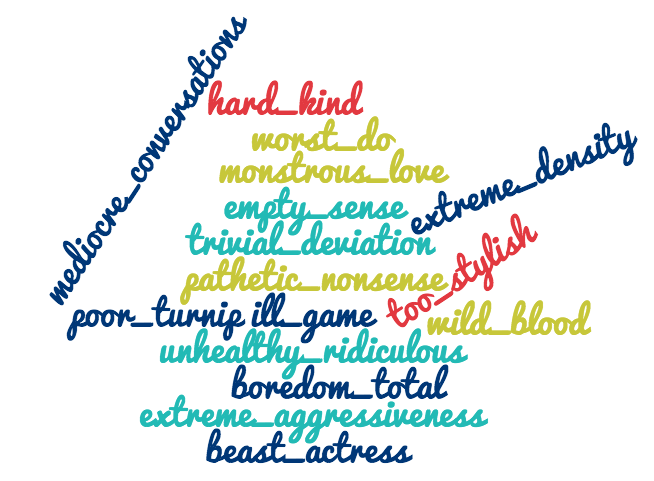
\includegraphics[width=7cm, height=5cm]{negative_en.png}
\end{figure}
\subsection{\textbf{What it gets Right or Wrong?}}
\indent If a sentence has a simple structure and is not contextually dependent on the previous statements, our model performs fairly good. For example,
\begin{enumerate} \item \textbf{The original text in French:} Ceci est un bon film avec des acteurs impressionnants. \textbf{\item A word-by-word gloss:} This East a good movie with of the cast impressive. \item  \textbf{A translation into English:} This is a good movie with awesome actors.
\end{enumerate}
\indent For sentences having a negation about an opinion or the ones in which the opinion contextually depends on the previous statements, the implementation does not give a correct output. For the below given example, our implementation identifies feature as "very good movie" but this is not contextually correct as per the overall review.
\begin{enumerate} \item \textbf{The original text in French:} Comme il était la suggestion de mon ami, je pensais que ce film serait très bon , mais il était pas à la hauteur de mes attentes.
\item \textbf{A word-by-word gloss:} As the  was the suggestion of my friend , l thought this movie would be very good, but its was not at the height of my expectations.
\item \textbf{A translation into English:}  As it was the suggestion of my friend , I thought this film would be very good, but it was not upto my expectations.
\end{enumerate}

\section{\textbf{Discussion}}
\indent We have summarized the reviews in French and German by identifying the relevant feature-descriptor pairs and classifying them as positive or negative. Evaluating the results we saw that our summarizer was able to identify most of the positive and negative features of a product for which the reviews statements had a simple parse tree. With more semantic analysis and greater contextual reference we can make our summarizer to work properly for reviews having contradicting sentiments. This can be done by finding contrasting conjunctions in sentences and figuring out if the noun they are referring to is the feature being analyzed. Along with that, we can identify sentence relationships showing contradiction in opinion about the feature and remove the feature-descriptor pair from consideration. This will improve our summarizer significantly.\\\\
\indent For future work, we plan to make it compatible for few other languages like Japanese and Hindi. This will help us to identify the positive and negative features of a product on a regional basis. As we know that an opinion may differ from person to person and from region to region, our summarizer can be of a great help while identifying which features are preferred in a place or a region and which are not. This could prove helpful for a manufacturer to decide which features to improve in the upcoming product versions in a geographically targeted manner.
Furthermore, we also plan to extend our summarizer to be capable of summarizing journals and newspapers. In this way we can even categorize the trending news and extract the good and bad happenings on a regional basis. It can be an exciting experiment to see what is the good work being done by a government/organization in a region and the decisions with which the citizens/employees are not satisfied.\\

\section*{\textbf{References}}
\begin{itemize}
\item Minqing Hu and Bing Liu. "Mining and summarizing customer reviews". Proceedings of the ACM SIGKDD International Conference on Knowledge Discovery \& Data Mining (KDD-2004, full paper), Seattle, Washington, USA, Aug 22-25, 2004.
\item Peter Prettenhofer and Benno Stein. "Cross-Language Text Classification using Structural Correspondence Learning". In 48th Annual Meeting of the Association of Computational Linguistics (ACL 10), pages 1118-1127, July 2010. Association for Computational Linguistics.
\item Amazon review dataset: http://www.uni-weimar.de/en/media/chairs/webis/corpora/corpus-webis-cls-10/
\item CLiPS pattern library for text analysis: http://www.clips.ua.ac.be/pattern
\item DISCO API to retrieve the semantic similarity between arbitrary words and phrases.
http://www.linguatools.de/disco/disco\_en.html

\end{itemize}
\section*{\textbf{Division of labour}}
\begin{itemize}
\item \textbf{Siddharth:} Sentiment \& Semantic Analysis, Performance Evaluation, Data Annotation.
\item \textbf{Piyush:} Dependency Parsing, Semantic Analysis, Performance Evaluation, Data Annotation.
\item \textbf{Susanth:} Data collection \& Preprocessing, Shallow Parsing, Data Annotation.
\item \textbf{Dishant:} Data Preprocessing, POS Tagging, Frequent Itemset mining, Data Annotation.
\end{itemize}


\textbf{Word Count:} 2094

\end{document}


